\documentclass[aps,prl,10pt,twocolumn,floatfix]{revtex4-2}
\usepackage{graphicx}
\usepackage{dcolumn}
\newcolumntype{d}{D{.}{.}{-1}}
\usepackage{url}
\usepackage{physics}

\bibliographystyle{apsrev4-2}


\begin{document}

\begin{abstract}
Kater's pendulum is a device that uses two moveable masses and two knife edges on a metal rod to measure the local value of gravity. 
This is accomplished by moving the two masses around on the rod to produce the same period when the rod is rotating in the up and down orientations, using the knife edges to pivot on a platform. 
This period value can then be used to calculate the local value of gravity.
From this experiment we found the local value of gravity at Starkville, MS to be $9.7912536(1002)m/s^2$, which is within $2\sigma$ of the local value, $9.7908(10)m/s^2$.
\end{abstract}


\title{Precise Measurement of Gravity Using Kater's Pendulum}
\author{C. T. Rochelle}
\email{ctr233@msstate.edu}
\author{K. J. Grimes}
\date{\today}
\affiliation{Department of Physics and Astronomy\\Mississippi State University\\Mississippi State, MS 39762-5167}
\date{\today}

\maketitle

\section{Introduction}\label{Intro}
% Lead Up to Creation
Prior to the creation of Kater's Pendulum, the best method for finding the local value of gravity was using a very light thread that was fixed at one end and a metal sphere tied to the other. 
This method yielded a value of gravity, although it had one major flaw, the inability to prevent energy loss due to angular momentum.
When the metal sphere swung from the thread, sometimes the sphere would wobble due to many external factors and cause some of the pendulum's energy to be lost to angular momentum \cite{BeforeKater}. 
% Invention
This reason caused captain Henry Kater to devise and create his own pendulum in 1817\cite{KatersWork}!
His new pendulum had two major improvements over the old design, both sides of the pendulum being fixed as to prevent energy loss due to angular momentum and the pendulum being compound. 
% How Does it Work
Instead of having to swing from a cord, the pendulum was solid metal rod, as to make no energy lost to angular momentum. 
This alone made the measurement much more precise!
The pendulum was also compound, meaning it has two weights, instead of one, that could offset each other and add more mass to the system to negate air friction and like retardant forces. 
The two weights consisted one one heavy, fixed one at one end and a small, movable one at the other. 
This allows the one small weight to be adjusted, either on a macro or micro scale, to influence the center of mass of the pendulum.

\section{Theory}\label{Theory}
% Derivation of Formula 
We know from the lab manual that ``if the period of oscillation of a physical pendulum about one axis a distance $l_1$ from the center of mass (i.e., the radius of gyration) is $T_1$ while the period of oscillation about the other pivot a distance $l_2$ from the center of mass is $T_2$, then the acceleration due to gravity is given by"
\begin{equation}\label{EQ1}
\frac{8\pi^2}{g}=\frac{T_1^2+T_2^2}{L}+\frac{T_1^2-T_2^2}{l_1-l_2}
\end{equation}
where $g$ is the local gravity, $T_1$ is the period measure of End A upright, $T_2$ is the period measure of End B upright, $L$ is the length of the rod, $l_1$ is the length to the adjustable weight from the top knife-edge, and $l_2$ is the length from the adjustable weight to the bottom knife-edge\cite{Manual}. 
This is true of all physical pendulums, although it requires the measurement of four different quantities to determine $g$, meaning more uncertainty would be introduced into the final value obtained for gravity than if we could reduce the amount of measurements being made. 
If we adjust the small, movable weight to make the periods, $T_1$ and $T_2$, equal each other, we can cancel one of the fractions and drop the number of values we must measure to 2!
The periods being equal makes equation \ref{EQ1} become
\begin{equation}\label{EQ2}
\frac{8\pi^2}{g}=\frac{2T^2}{L}+0
\end{equation}
where $T=T_1=T_2$.
We can now rearrange equation \ref{EQ2} to solve for $g$
\begin{equation}\label{finalE}
g=\frac{4\pi^2L}{T^2}
\end{equation}

\section{Experiment}
% What did you do?
\begin{figure}
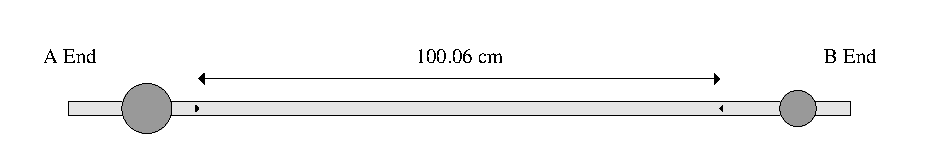
\includegraphics[width=230px]{diagram.eps}
\caption{This figure is a schematic of the Kater's Pendulum device. Three important notes are the two masses at each end (the B side mass is movable), the two knife edges at end end, and the distance between the knife edges being a known $100.06(10)$cm.}
\label{pendulum}
\end{figure}

At the heart of the Kater's Pendulum experiment is the Kater's pendulum device, seen in Figure \ref{pendulum}. 
This device is a metal bar that has two knife edges 100.06(10)cm apart pointing towards the center of the rod and two moveable masses positioned passed the knife edges on each end. 
This is placed on a metal hook protruding from the wall that it is allowed to pivot on. 
The bigger mass on End A of the pendulum was placed 15.0(1)cm from the top knife edge, where it remained for the duration of the experiment. 
The smaller mass on End B of the pendulum was initially placed at 53.0(1)cm from End A's knife edge, the reference point for the initial round of data collection. 
Even though the knife edge on End A came to a sharp point, some lubricant was required at the pivot location to reduce energy lost to friction. 
At End A and End B of the pendulum there were toothpicks protruding from the middle of the metal rod to allow for more precise data collection of the period in the photogate. 

The entire apparatus described so far was hanging and pivoting above the photogate sensor which connected to the PASCO Capstone software on a nearby computer to collect data about the time and period of the oscillations. 
An important note about data collection is that we used the PASCO software to only account for one in every ten periods of oscillation to improve the precision at which the computer was able to take the data.
This was later factored out of the equation, while still keeping the higher precision, by dividing our value by ten. 

This experiment was divided into two parts. 
This first part entailed trying to find an approximation to where the two periods would equate.
We needed to approximate this point so that we could come back later and take more data around the area of interest.
The second part is a more precise analysis to determine a more accurate location for the cross.

In the first section we took twenty data sets, ten with End A upwards and ten with End B upwards. 
Each data set contains ten data points that were taken during the three and a half minute duration of each set.
Each set started with an original oscillation amplitude of 2.0(2)cm.
Each data series for the pendulum (being each orientation) started at 53.0(1)cm from End A's knife edge and was increased in distance by 10cm each sequential data set, going all the way to 153(1)cm. 

After all the data was collected, data analysis began and resulted in Figure \ref{1stGraph}.
The dotted lines were generated by preforming a least-squares polynomial fit on each group of data.
As seen from Figure \ref{1stGraph}, there are two intersection points, meaning the periods would be equal at those points.
One of those two points is the area of interest for the second portion of this lab.
We chose to look further into the rightmost intersection point to allow us to move the smaller weight with less adjustments.

For the second part of the experiment, we preformed a similar routine to the first, although in more detail to allow for a more precise intersection point. 
From Figure \ref{1stGraph}, we saw the intersection point was somewhat around $130cm$, and we centered our second experiment around that point. 
For each orientation of the device we took nine measurements, starting at $126(01)cm$ and increasing by $1(01)cm$ until hitting $134(01)cm$. 
This was done for both orientations. 

For the specifics of the data collection, we used a caliper to precisely measure the locations and increments on the device using a pen.
We also collected all data at night to avoid the amount of external vibrations generated by doors closing or people jumping in the building. 
For each data set we started the oscillations with an amplitude of $2.0(2)$cm and allowed the pendulum to run for thirty minutes without collecting any data for any inconsistencies or wobble to be removed from the system. 
After the first thirty minutes was up, we collected data for the following thirty minutes, using the same program described in the first part. 


\section{Data Analysis}
% Explain the Results 
\begin{figure}
\includegraphics[width=230px]{FirstMeasurement.png}
\caption{This figure shows a plot of our first section of our experiment in the form of a period [s] versus distance [cm] plot. The solid dots are the averages of the periods taken for the duration of each data set. The dotted lines is the fit generated by the least-squares polynomial fit. The blue data points and line represent the pendulum with End A upwards and the orange data points and line represent the pendulum with End B upwards.}
\label{1stGraph}
\end{figure}

For the first section of the experiment, we preformed an unweighted average on each data set to receive the averages that were plotted in Figure \ref{1stGraph} and shown in Table \ref{1stTable}.
A polynomial least-squares fit was preformed using the averages to generate the two curve fits shown on Figure \ref{1stGraph}. 
This first section was only a rough estimate so we simply looked where the lines looked to have crossed and chose a point around that, in our case $130cm$. 

\begin{figure}
\begin{tabular}{|c|c|c|}
\hline
& \multicolumn{2}{|c|}{Periods [s]}\\
\hline
Distance [cm] & End A Upwards [s] & End B Upwards [s]\\
\hline
53&	2.1148&	2.1116\\
63&	2.0798&	2.0959\\
73&	2.0570&	2.0875\\
83&	2.0453&	2.0798\\
93&	2.0429&	2.0787\\
103&	2.0513&	2.0801\\
113&	2.0659&	2.0863\\
123&	2.0885&	2.0976\\
133&	2.1161&	2.1134\\
153&	2.1867&	2.1587\\
\hline
\end{tabular}
\caption{A table of the data set averages collected during the first section of the experiment. There are no uncertainties because this is simply the rough data to find around where the two lines cross.}
\label{1stTable}
\end{figure}

There is an important note on the second data. 
In the Capstone software, we set up the second set to include an extra digit of precision by using the computers clock speed instead of the time set on the system;
however this extra digit was lost during an export of our data and could not be recovered.
This extra point of precision would have been useful to have during the second round of analysis;
however it was not necessary, so we continued without it.
Some of the precision was brought back from taking the difference between every other value of the time between ten swings.

The second part of the experiment was analyzed using a linear least squares fit, using the period data and distance from the reference point. 
Every data set was divided up and a chi-squared minimization was preformed on all of the eighteen of the sets to arrive at the y-coordinate of the linear fits, which are shown in Table \ref{2ndTable}.
An important point is that the $+3cm$ data point for End A Upwards was a significant outlier, differing from the other points by 5 sigma, and was removed for this reason.
This may be the result of faulty analysis or data measurement being off. 

\begin{figure}
\includegraphics[width=230px]{SecondMeasurement.png}
\caption{This figure shows the plot from our section round of data collection in the form of a plot of period [s] versus distance [cm]. The solid blue and orange data points show the chi-squared fit's slope values. The dotted lines show the least-squares polynomial fit. The blue points represent the pendulum with End A up, and the orange points represent End B up. There are error bars included in this graph; however, most are so small that they are covered up by the data points themselves. }
\label{2stGraph}
\end{figure}

The linear regression was now preformed on the data set and yielded the trend lines shown in Figure \ref{2stGraph} and the values shown in Table \ref{2ndTable}.
From the equations of the trend lines we can find a precise point of intersection.
If we remember from the theory section, this is the point that the two periods become the same value and can be substituted into Equation \ref{finalE} to solve for the local value of gravity in Starkville, MS. 

Using the period value obtained from the second data analysis , $2.0085885(6)s$, we come to a final value of gravity in Starkville to be $9.7912536(1002)m/s^2$. 
The accepted value for gravity in Starkville is $9.7908(10)m/s^2$.
Our value falls within the the uncertainty of the accepted value!
An important note about the uncertainty in our value is that the uncertainty in the length of the rod was three orders of magnitude off of our uncertainty for the period, making the uncertainty in the rod dominate the uncertainty of our measured value of gravity.  

\begin{figure}
\begin{tabular}{|c|c|c|}
\hline
& \multicolumn{2}{|c|}{Periods [s]}\\
\hline
Distance [cm] & End A Upwards [s] & End B Upwards [s]\\
\hline
-4&	1.996266(38)&2.001301(8)\\
-3&	1.999025(8) &2.003088(8)\\
-2&	2.001301(8) &2.004612(8)\\
-1&	2.003088(8) &2.006479(10)\\
0&	2.006441(8) &2.007951(8)\\
1&	2.009461(8) &2.010073(8)\\
2&	2.013027(8)&2.009461(8)\\
3&	--- &2.011306(8)\\
4&	2.018746(8) &2.013028(8)\\
\hline
\end{tabular}
\caption{A table of the data set averages collected during the second section of the experiment, with $0cm$ offset being at the $130.85cm$ position on the rod.}
\label{2ndTable}
\end{figure}


\section{Conclusion}
% Conclusion 
From the Kater's Pendulum experiment, the value we obtained fell within the $2\sigma$ range of the local value of gravity.
however this could be improved by a lot!
One of the main catastrophes that happened during this experiment was the loss of one of the time digits in the second round of data collection. 
This extra digit could dramatically improve the uncertainty related with the our value.
An easy fix would be permanently fixing the toothpicks at the end of the device.
Sometimes these would be bumped or move throughout the experiment and we would have to reset them in their place.
This could account for some of the variability in times during our experiment. 
Another major improvement to our experiment could be varying the amount of time we allowed the pendulum to stabilize between End A and End B being up.
Looking at Figure \ref{2stGraph}, we see that the values for End B being up had significantly less deviation from the trend line as compared to End A being up. 
One of the most probable reasons is the time taken for the pendulum to stabilize given the orientation of the movable masses. 
When End B is upwards, the larger mass travels more distance during each gyration, stabilizing the system faster then when the smaller mass is on the bottom, when End A is upwards. 
To correct for this, we should have allowed for more stabilization time when End A was upwards to allow the system to stabilize more, giving more precise values of period. 
As we mentioned in our conclusion, the uncertainty in our measurement of gravity could also be improved drastically by obtaining a more precise distance between the knife edges.
As a side note, we could also use a Gravimeter to easily and more accurately measure the local value of gravity in Starkville.
But where is the fun in that.

\begin{thebibliography}{9}
\bibitem{BeforeKater} Britannica, T. Editors of Encyclopedia. \textit{pendulum} (Encyclopedia Britannica, September 1, 2021). \url{https://www.britannica.com/technology/pendulum}.
\bibitem{KatersWork} H. ~Kater, \textit{An Account of Experiments for determining the Length of the Pendulum Vibrating Seconds}, (The Latitude of London, 1817).
\bibitem{Manual} J. ~Winger, \textit{Precise Measurement of g Using Kater’s Pendulum}, (Mississippi State University).
\end{thebibliography}

\end{document}
